\section{The ULTRACAM instrument} 

The ULTRACAM high speed photometry camera (hereafter, ULTRACAM) had its `first-light' at the William Herschel Telescope (WHT) on the 16 May 2002. Since then it has been used on many occasions at three telescopes, namely the William Herschel Telescope (WHT), La Palma, Islas Canarias, the Very Large Telescope (VLT), Cerro Paranal, Chile and New Technology Telescope (NTT), La Silla, Chile. The camera is designed to be portable and can travel between these telescopes. It was designed specifically to take high speed photometry of faint objects in three colours. These three factors are fundamental to understanding the scientific value of ULTRACAM and also set important context into the reason for doing this project, so let's first discuss each one in turn. 

\subsection{"High speed"}

\subsection{"Faint objects"}
ULTRACAM was designed to be installed on some of the larger telescopes in the world. The WHT has a mirror diameter of 3.5 metres, NTT xx metres and the VLT 

\subsection{"Three colours"}
In Astronomy, colour is an important property that can tells a great deal about the object. 

\section{Candidate objects}

One of the main reasons for automating the pipeline is that we might, serendipitously, discover objects that are showing variability, that were not the intended target of the run. Depending on the choice of windows that the observer has selected and how crowded the sky in the field of view happens to be, we could have many objects recorded in the raw data that have not had light curves produced. Producing and analysing these new light curves will hopefully allow us to discover new variable objects. 

Due to the nature of the exposure times and the run lengths (discussed in the previous sections), we are limited to picking up objects that have a variability that occurs within a few minutes to a few hours. We list below that types of objects that we expect to discover.

\subsection{Eclipsing binaries}
Binaries stars that have their orbit inclined towards Earth ($i \sim 90^\circ$) such that eclipses will occur at least once per orbit will show a change in flux that will be detected in the ULTRACAM data. Our typical run length of 1-3 hours favours binaries that have a short period (\textless 1 day). 

\subsection{Contact binaries}
Contact binaries are star systems where at least one of the stars has filled its Roche lobe and the stars are effectively 'in contact' with one another, allowing matter to flow, in at least one direction. 

\subsubsection{{W UMa} stars}
{W UMa} stars are binaries where both stars are in contact with each other. Also, each star in the contact binary is significantly distorted, resulting in ellipsoidal variations of the flux due to the fact that the projected area of the stars is constantly changing. Their periods fall in the 6 to 20 hours range and should therefore be clear in a typical ULTRACAM run lasting for, say, 30 minutes or more. 

Need a reference for a {W UMa} review article.

\subsubsection{Other contact binaries?}
Anything else here?

\subsection{Cataclysmic variables}
Cataclysmic variables are highly variable on many different timescales. On the timescale of centuries, they can undergo \emph{nova} where they explode a shell of hydrogen that has been built up on their surface, increasing their brightness by 6-19 magnitudes. Over a period of weeks to months, their accretion disks can go into \emph{outbursts} increasing their magnitudes by a few magnitudes. On the timescale that is most relevant to a typical ULTRACAM run, we can expect to see eclipses of the white dwarf, bright-spot and disc (assuming this is an eclipsing system, with an appropriate orbital inclination) and flickering caused by the accretion stream flowing onto the bright-spot. 

Reference to Coel Hellier's book here (or Brian's book). 

\subsection{Intrinsic variables}

\subsubsection{RR Lyrae stars}
A bit about RR Lyraes and how we might see them in the ULTRACAM archive.

\subsubsection{$\delta$ Scuti stars}
A bit about $\delta$ Scuti stars and how we might see them in the ULTRACAM archive.

\subsubsection{DAV and DBV stars}
A bit about pulsating White Dwarf stars and how we might see them in the ULTRACAM archive.

\subsection{Flare stars}

Flare stars are usually red dwarf or brown dwarf stars that undergo flares in their atmospheres resulting in rapid changes in brightness on timescales of minutes to hours. This obvious change in brightness should be detected during an ULTRACAM run. 

\subsection{Near Earth objects}
Near Earth objects, such as asteroids and Kuiper belt objects should be visible in the ULTRACAM archive. Asteroids are likely to move across the field at a few arc seconds per minute, meaning that they would cover a fair fraction of the exposed image during the course of a 1-2 hour run of the ULTRACAM. Kuiper belt objects will have magnitudesof around ?? and would move only a few arcseconds per hour.

\subsection{Optics}

The camera has three CCD detectors enabling it to capture data in three colour bands simultaneously. Two dichroic beamsplitters divide the light from the collimator into three beams, which shall hereafter be referred to as the `red', `green' and `blue' channels. The three CCD detectors are mounted at right angles to each other on the camera. Therefore, each detector is at the end of a slightly different optical path. The images produced on each of the three CCDs chips are therefore of the same field but with very slightly different orientations, distortions and offsets. Towards the edges of the chips, these differentials can add up to be on the order of 10 pixels from channel to channel. 

While the exposure timing is synchronised across the detectors, it is, however, possible to have the detector in the blue channel remain exposed and not 'read-out' while the other two are going through multiple exposures and 'read-outs'. This is to allow for longer exposures where there might be less flux in blue. Reduced flux in blue is caused by several factors, including lower transmission of the optics and atmosphere to blue light, the reduced sensitivity of the CCD detector to blue light and the intrinsic flux of most astronomical objects is lower in this channel.

\begin{figure}[!h]
\centering
\includegraphics[width=90mm]{images/IMG_0121_scaled.JPG}
\caption{The Ultracam being commissioned in May 2002.}
\label{fig1}
\end{figure}

\subsection{Filter sets}
The filters for each channel can be altered by the observer. In usual configurations, the SDSS filters (u, g, r, i, z) are used, but there are a selection of narrow-band filters that can be substituted. Depending on the science measurements that the observer is trying to perform, these filters will be changed.   

\subsection{Field size and pixel scale}
ULTRACAM is usually mounted on one of the three telescopes mentioned in the introduction of this chapter. Field sizes, pixel scales and orientations are summarised in the table below. The orientations quoted refer to when the camera is \emph{not} rotated.

\begin{center}
\begin{table}
	\begin{tabular}{|l|r|r|r|}
    	\hline
		Telescope & Field size (arc minutes) & Pixel scale (arc seconds/pixel) & Orientation \\
		\hline
		WHT & 6.0x6.0 &  0.35 & N(up), E(left)\\
		NTT & 6.0x6.0 & 0.35 & N(up), W(left)\\
		VLT & 2.5x2.5 & 0.15 & N(up), E(left) \\
		\hline
	\end{tabular}
	\caption{The field sizes and pixel scales of ULTRACAM on each of the three telescopes. }
	\label{tab:pixelscale}
\end{table}
\end{center}
Comment: Confirm these figures with Tom/Elme.


\subsection{High speed operation}
A key aspect of the design of the camera is its ability to perform at high cadence. It is possible to have the camera read-out at up to 500Hz (frames per channel per second) \cite{dhillon07}. This makes the camera useful for observations of rapid transient events with accurate timing. Although the camera is not often used in this very high speed mode, there are a few observing runs where the camera has been operating with exposure times of approximately 0.005 seconds. These runs are described in chapter~\ref{chap:results}.

Each CCD has a total pixel area of 2057x1024 pixels. Half of these pixels are masked and never exposed to light. They are used as a temporary buffer for reading out the chip. CCD detectors are read out serially, but in order to decrease the time between exposures, the full image can be moved to the blanked out area of the chip and this can then be read out while the un-masked area of the chip is once again exposed to light. 

\begin{figure}[!h]
\centering
\includegraphics[width=90mm]{images/ccd.png}
\caption{One of the three CCD detectors. The masked-off area is visible in the lower half of the chip surface.}
\label{fig2}
\end{figure}

ULTRACAM gives the observer the option to reduce the area of the detector that is used for the exposure. This reduces the readout time of the chip and enables the high cadence. Reducing the number of pixels exposed also decreases the amount of data storage needed for the run. The observer can define pairs of \emph{windows} that are centered on their objects of interest. By making the windows suitably small, the observer can use the camera in extremely high cadence mode. 

The highest cadence mode is called \emph{Drift mode}. This mode uses the masked area of the CCD chip to store several exposures simultaneously. Only the portion of the CCD that is exposed is shifted into the masked area of the CCD meaning that the unmaksed area is ready to be re-exposed more quickly. This mode requires that only the lower portion of the detector, close to the boundary of the masked and un-masked areas, is exposed. Due to the geometry of this readout mode, it is necessary that the exposed area of the CCD is immediately adjacent to the boundary with the masked-off section of the chip. This means that the camera will have to be rotated so that the target object (and a suitable comparison star) are positioned correctly. The ULTRACAM is therefore designed to be rotated. For any particular run, it is possible that we can have \emph{any} orientation ($0-180^{\circ}$) of the camera relative to the sky coordinates. The ULTRACAM logs do not record this rotation angle. This is an important factor to remember when we try to find astrometric solutions for the runs.    

\begin{figure}
  \centering
  \setlength{\fboxsep}{0pt}
  \setlength{\fboxrule}{1pt}
  \fbox{\includegraphics[width=120mm]{images/run010_r_inverted.png}}
  \caption{A 'fully' exposed CCD with 1 pair of windows (512x1024 pixels each).  This mode reads out the full area of the CCD chip, resulting in larger data sizes and a longer readout time. The field of view is approximately 7x7 arc minutes, but varies a little depending on the telescope that the camera is mounted on.}
  \label{fig:KOI-824}
\end{figure}

\begin{figure}  
  \centering
  \setlength{\fboxsep}{0pt}
  \setlength{\fboxrule}{1pt}
  \fbox{\includegraphics[width=120mm]{images/run016_r_inverted.png}}
  \caption{A 'masked' exposure with 2 pairs of windows (350x300 and 250x250 pixels each, respectively)}
  \label{fig:V713Cep}
\end{figure}

\begin{figure}  
  \centering
  \setlength{\fboxsep}{0pt}
  \setlength{\fboxrule}{1pt}
  \fbox{\includegraphics[width=120mm]{images/run018_r_inverted.png}}
  \caption{The camera operating in \emph{drift-mode}. Note the very small windows (172x156 pixels) located at the bottom of the imaging area.}
  \label{fig:V834Cen}
\end{figure}

More details on the camera design and operation can be found in \cite{dhillon07}.

\section{ULTRACAM data}

\subsection{Data capture}
Usually the camera remains installed on the telescope for a week or so and is used for observations on consecutive nights. Each separate recording of data is called a \emph{run}. On most nights, many \emph{runs} are recorded. A \emph{run} can be defined as a period when the camera is active and gathering data. Not all runs are used for gathering \emph{scientific} data. Some runs are used for target acquisition and camera calibration purposes. 

The types of runs are: 
\begin{itemize}
	\item \emph{Science run}: These are the runs that contain the valuable scientific data. They usually comprise the longest portions of the observations during the night, unless the camera is having difficulties or adverse conditions are preventing useful astronomical observations.
	\item \emph{Acquisition run}: These are runs, usually of short duration (ie a few minutes) during which the telescope is being moved in order to place the candidate object(s) in the field of view. The camera may also be rotated in order to align the CCD such that the targets avoid `bad' pixels or are near to the lower boundary of the detector (eg for high speed readout in Drift mode). 
	\item \emph{Flat field}: At the start and the end of the night (usually during twilight) the observer will take a few runs to create \emph{sky-flats} that will be used later for calibrating the variations in pixel sensitivity across each of the detectors.  Sky-flats are generated by exposing the camera to patches of sky during the twilight. 
	\item \emph{Bias}: A short run to build calibration readings for measuring the bias of the detector. This bias will be subtracted from the data during the reduction. 
	\item \emph{Timing calibration run}: One way to check the timing measurments of the camera is to take frames of a well-known rapidly oscillating source. For example, the Crab Pulsar (PSR B0531+21). The timing of the pulses as measured by the camera can be compared to the expected times for the pulsar. This is used as a standard clock for timing calibration.
\end{itemize}

\subsection{Typical run length}
Since ULTRACAM is designed for high-speed photometry, observers using the instrument are typical looking for variations that are clearly noticeable on timescales from a few minutes to a few hours. Most science runs are last for a few hours at the most. The longest runs are usually observations of exoplanet transits. These runs can last 4-7 hours. Very often they have a break in the middle of the run where the telescope has reached the zenith and the run is interupted since the telescope cannot observe at the zenith due to the alt-az mount design.  

A look at the distribution of run length shows a large bulk of the runs are shorter than 5 minutes. This is because there are far more acquisition runs, flat-fields and bias runs than there are science runs. There are also many runs that are nominally science runs (and can be used as such) but are short because the observer has noticed something that they would like to change. This could be a change in focus, binning factor or integration time. The run is then cut short and a new run is started. The longest run length in the 10 year data archive is 566 minutes or 9.5 hours, taken on 25th of April 2010 at the NTT. This was for the observation of a transit of the exoplanet Wasp-15b. The output for this run can be seen at \small \url{http://deneb.astro.warwick.ac.uk/phrnaw/sitedev/2010-04-25/run020.html}. 

\begin{figure}[!h]
  \centering
  \includegraphics[width=120mm]{images/hist0-600.eps}
  \caption{Distribution of run length. Many runs are shorter than 5 minutes, but these are not usually \emph{science runs}.}
  \label{fig:histogram0-600}
\end{figure}

\begin{figure}[!h]
  \centering
  \includegraphics[width=120mm]{images/hist10-600.eps}
  \caption{Distribution of run length after removing runs shorter than 10 minutes.}
  \label{fig:histogram10-600}
\end{figure}

\begin{figure}[!h]
  \centering
  \includegraphics[width=120mm]{images/hist60-600.eps}
  \caption{Distribution of run length after removing runs shorter than 60 minutes.}
  \label{fig:histogram60-600}
\end{figure}


\begin{figure}[!h]
  \centering
  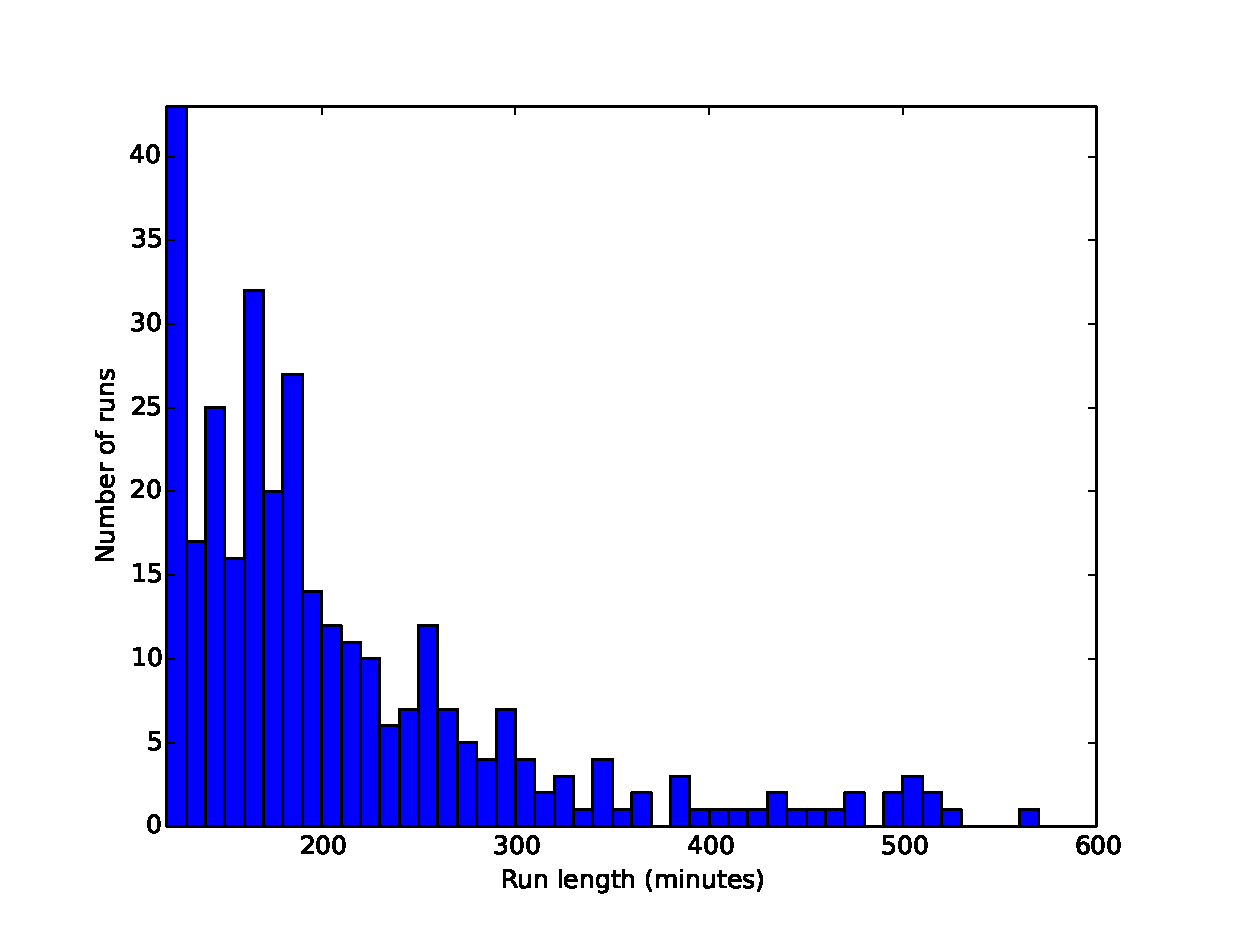
\includegraphics[width=120mm]{images/hist120-600.eps}
  \caption{Distribution of run length after removing runs shorter than 120 minutes.}
  \label{fig:histogram120-600}
\end{figure}

\subsection{Run cadences}
As mentioned in the section describing the camera, ULTRACAM was designed specifically for high-speed photometry. This allows a relatively un-explored region of the observational parameter space to be opened up. Certain phenomena in astrophysics have observables that take place in short periods. Ultra-compact binaries, Cataclysmic variables, Neutron stars, etc all have signals that can be resolved at even sub-second intervals. ULTRACAM is also mounted on some relatively large telescopes, with mirrors ranging from 4.2m 8.2m in diameter. This means that it is able to perform high speed photometry of relatively faint objects. Since the commissioning of the camera in 2002, it has been used to observe a variety of objects, summarised in table \ref{tab:breakdown}. 

Only certain objects require the highest cadences (\textless 1 second). These are X-ray binaries, Polars, Pulsars, Flare stars. Many other science runs can use the camera with a \textgreater 1 second exposure time. Long runs for exoplanet transit observations often use longer exposures of 2-3 seconds. The longest exposure times are around 20-25 seconds. This is only required when the object being observed is extremely faint.  

\begin{table}
  \begin{center}
	\begin{tabular}{|l|r|}
		\hline
		Target & Time (percent) \\
		\hline
		Cataclysmic Variables & 25.3 \\
		X-ray binaries & 17.4 \\
		sdB stars/asteroseismology & 11.2 \\
		etc & x.y \\
		\hline
	\end{tabular}
  \end{center}
\label{tab:breakdown}
\caption{Breakdown of how ULTRACAM is used. Comment: This is the out of date table from \cite{dhillon07}. Should update this.}
\end{table}


\begin{figure}[!h]
  \centering
  \includegraphics[width=120mm]{images/cadences_hist0-25.eps}
  \caption{Distribution of exposure times used in the \emph{science} runs.}
  \label{fig:cadences}
\end{figure}

Figure \ref{fig:cadences} shows a distribution of exposure times by run, for all of the \emph{science} runs in the ULTRACAM data archive. There are several groupings apparent in the histogram. Firstly, the very short exposures for the rapidly variable objects, such as Polars, Pulsars and X-ray binaries. Then there is a cluster of runs with exposure times of 2, 3, 4 and 5.5 seconds. These are typically observations of eclipsing binaries. The next cluster occurs at about 10 seconds, which are usually runs for exoplanet transits. The final cluster of run lengths occurs at around 20 seconds, usually reserved for faint objects.

\begin{table}
  \begin{center}
	\begin{tabular}{|l|r|}
		\hline
		Exposure time (seconds) & typical target \\
		\hline
		0-1 second & X-ray binaries, polars, CVs \\
		2, 3, 4, 5.5 seconds & eclipsing binaries, exoplanet transits \\
		10 seconds & exoplanet transits \\
		25 seconds & faint objects \\
		\hline
	\end{tabular}
  \end{center}
\label{tab:breakdown}
\caption{Typical exposure times and the type of target being observed. Comment: Characterisation here is not thorough. Will clean it up if this table is valuable.
}
\end{table}

\subsection{The data archive}
At the time of writing, the ULTRACAM data archive comprises of about 10 terabytes of saved data. This can be broken down as:
\begin{itemize}
	\item \emph{406} nights on which ULTRACAM was operational at a telescope.
	\item \emph{12 649} runs, including science runs, acquisition runs, flat fields and biases. 
	\item \emph{119 817 742} frames in total. This total includes all the frames for each channel: red, green and blue.
	\item \emph{10 542 378 791 454} bytes or 10.54 terabytes of raw image data.
\end{itemize} 

The data set is relatively large and is housed on a network mounted storage device that is only available through the internal university computer network. This means that it is not possible to access this data from remote locations (for example, by research collaborators in different institutions). If a researcher needs to see some data, then they need to contact a member of department at Warwick or Sheffield and request a data reduction. There is no means to explore the ULTRACAM data set from a remote location. Providing a simple means of accessing the data from remote locations would benefit all of the research collaborators. 


